\documentclass[11pt]{article}
\usepackage{anysize}
\usepackage{graphicx}
\marginsize{1 in}{1 in}{0.5 in}{6 pt}
\title{CMSI 370-01 Assignment 0918}
\author{Chris Whiting}
%\setlength{\intextsep}{-0.5ex}
\begin{document}
\maketitle

For our experiment, we wanted to test the learnability, efficiency, and satisfaction of HBO GO and Netflix. We ran four tests in order to rate and record each of these metrics. The Learnability of a system is the time it takes to accomplish a task with that system from a subject who is unfamiliar with the system. The Efficiency of a system is the time it takes to accomplish a task with that system from a subject who is familiar with the system. The last metric to be considered while running our tests was Satisfaction, which is the rating at which each subject either enjoyed or hated performing tasks on the system. 
 
\begin{verbatim}
TEST 1: Search Movies/TV Shows
\end{verbatim}
Our first test is to search for a certain movie or tv show and although HBO Go and Netflix have a different selection, we can still perform accurate tests because we are not testing for each sites' selections. We timed each participant on how fast this task could be accomplished. 

\begin{table}[ht]
\caption{Movie/TV Show Results} % title of Table
\centering % used for centering table
\begin{tabular}{|c|c c c c| c |}  %ADD MORE COLUMNS HERE
\hline\hline %inserts double horizontal lines
HBOGO show  &Justin& Mikey&Kevin&Travis&Average  \\ [0.5ex] % ENTER MORE SUBJECTS HERE
%heading
\hline % inserts single horizontal line
Black Swan  & 8.6s & 9.5s&6.1s &11.4s&8.9s    \\ %ADD MORE TIMES HERE
Entourage &9.7s&8.1s&9.0s &21.31s&12.0s  \\
Game of Thrones &6.5s&7.0s&6.9s &5.6s&6.5s \\ 
\hline %inserts single line
Netflix show &Justin& Mikey&Kevin&Travis&Average   \\ [0.5ex]
\hline
Adventureland &5.0s&8.5s&6.5s&6.1s&6.5s   \\
Scary Movie &5.0s&7.3s&6.5s&6.5s& 6.3s    \\
River Monsters &5.0s&6.2s&6.5s&4.8s&5.6s      \\
\hline
\end{tabular}
\label{table:nonlin} % is used to refer this table in the text
\end{table}

\begin{verbatim}
TEST 2: Video Navigation
\end{verbatim}
Video navigation categorizes our second test, where we timed how long each person took to fast forward from the start of a tv show up to around 15 minutes. Also the time it took to navigate to the next episode in line was recorded.

\begin{table}[ht]
\caption{Video Navigation Results} % title of Table
\centering % used for centering table
\begin{tabular}{|c| c c c c |c|} % centered columns (4 columns)  %ADD MORE COLUMNS HERE
\hline\hline %inserts double horizontal lines
HBOGO  &Justin& Mikey&Kevin&Travis&Average   \\ [0.5ex] % ENTER MORE SUBJECTS HERE
%heading
\hline % inserts single horizontal line
GOT 15min FF  &12.2s & 9.9s&7.3s&3.5s&8.2s     \\ %ADD MORE TIMES HERE
GOT (ep6 - ep7) &19.9s&21.8s&26.9s&27.6s&24.1s   \\ 
\hline %inserts single line
Netflix &Justin& Mikey&Kevin&Travis&Average    \\[0.5ex]
\hline
River Monsters 15min FF &6.0s&7.0s&5.2s&4.8s&5.8s \\
River Monsters (ep1 - ep2) &5.7s&6.3s&9.9s&3.9s&6.45s    \\
\hline
\end{tabular}
\label{table:nonlin} % is used to refer this table in the text
\end{table}


\begin{verbatim}






TEST 3: Genre/Filter Search
\end{verbatim}
For this test, we timed how long it took each participant to go from the home page of the website to a web page with only movies of that specific genre. We timed for comedy and romance movies. HBO GO has a dedicated Comedy button from the home page, but most people did not see this. 

\begin{table}[ht]
\caption{Filter Search for Movies Results} % title of Table
\centering % used for centering table
\begin{tabular}{|c|c c c c|c|}   %ADD MORE COLUMNS HERE
\hline\hline 
HBOGO  &Justin& Mikey&Kevin&Travis&Average   \\ [0.5ex] % ENTER MORE SUBJECTS HERE
%heading
\hline 
Comedy  &11.0s & 14.7s&12.9s&7.6s&11.6s  \\
Romance &4.6s&60.0s&8.8s&5.5s&19.7s    \\
\hline
Netflix &Justin& Mikey&Kevin&Travis&Average     \\ [0.5ex]
\hline
Comedy &9.6s&13.6s&9.5s&2.4s&8.8s   \\ %ADD MORE TIMES HERE
Romance &4.1s&N/A&9.7s&2.6s&5.5s  \\ 
\hline %inserts single line
\end{tabular}
\label{table:nonlin} % is used to refer this table in the text
\end{table}

\begin{verbatim}
TEST 4: Cast Member Search
\end{verbatim}
Searching for the web page with the cast and crew of a particular movie or tv show was the last test we timed. We had two movies/tv shows for each website and we timed how long it took each person to navigate from the home page to the page with the cast information.

\begin{table}[ht]
\caption{Filter Search for Movies Results} 				% title of Table
\centering 									% used for centering table
\begin{tabular}{|c|c c c c|c|} % centered columns (4 columns)  %ADD MORE COLUMNS HERE
\hline\hline 									%inserts double horizontal lines
HBOGO  &Justin& Mikey&Kevin&Travis&Average  \\ [0.5ex] 	    % ENTER MORE SUBJECTS HERE
%heading
\hline 									    % inserts single horizontal line
Black Swan  &16.8s & 18.5s&12.4s&15.8s&15.9s          \\			 %ADD MORE TIMES HERE
Hesher &9.5s&7.5s&6.7s&5.7s&7.4s                             \\
\hline
Netflix &Justin& Mikey&Kevin&Travis&Average   \\ [0.5ex] 			% [1ex] adds vertical space
\hline
Adventureland &9.0s&11.6s&10.5s&11.7s&10.7s          \\
True Grit &7.2s&15.1s&7.2s&9.9s&9.9s                         \\
\hline 										%inserts single line
\end{tabular}
\label{table:nonlin} % is used to refer this table in the text
\end{table}

\begin{verbatim}
SATISFACTION
\end{verbatim}
At the end of each test we asked each person to rate the websites from 1 to 10, 10 meaning using that particular site was very satisfying and 1 being not satisfying. Based on Table 5 below, our test subjects favored HBOGO slightly more than Netflix. They said that "HBO GO was easier to navigate" and "HBO GO looked prettier than Netflix". Also, based on the UI of each website, the HBOGO website is less cluttered with icons, advertisements, and miscellaneous buttons, which may have attributed to its higher satisfaction rate.

Based on the results in Table 1, it can be seen that searching for movies or tv shows is on average 2 seconds faster on Netflix than HBO GO. Also, a new user to HBO GO, Travis, was considerably slower than a new user to Netflix, Mickey, while searching. This suggests for test 1, that searching for movies and tv shows is both more learnable and efficient on Netflix than HBO GO.

Table 2 indicates that HBO GO is slower at video navigation to new and old users alike. An old user to HBO GO, Mikey, had trouble getting from episode 6 to episode 7 of Game of Thrones, as the test suggests. Also, Justin, a new user had trouble with this same test on HBO GO, but not Netflix. Where it took him 19.9 seconds to perform the next episode test in HBO GO and only 5.7 seconds in Netflix. This indicates that HBO GO is less learnable and efficient than Netflix, by a 15 second average margin. 

The third test was used to indicate which video-streaming application had the best genre search. Table 3 shows that when searching for either comedy or romance movies, HBO GO was 8 seconds, on average, slower than Netflix. Mikey, the old user to HBO GO took longer to perform this test, than he did with Netflix. This result suggests that Netflix is much learnable and efficient in this test category.

The fourth test gave similar results to both HBO GO and Netflix. For HBO GO, the first cast member search was for Black Swan and provided slow results for old and new users alike. However, the second cast member search for Hesher yielded results that were twice as fast. This can be attributed to HBO GO's high learnabliltiy in this subject. For Netflix, the average for both cast member searches was slightly faster than HBO GO's. However, the speed of the second test was only a second faster than the first Netflix test. Therefore, for test 4 the cast member search, HBO GO yielded higher learnablilty, while Netflix resulted in higher efficiency than HBO GO.

 HBO GO and Netflix are two video-streaming applications whose efficiency, learnablity, and satisfaction were tested by the four tests above. For this type of system, efficiency should be prioritized, because when a user wants to watch a movie, they do not want to wait.  A user, most of the time, has not seen the movie or tv show that they are trying to find on a video streaming application. Therefore, if the movie or tv show is not good, they do not want to take all day trying to figure out the video streaming service in order to pick another movie. At the end of the day, the time spent watching the movie rather than searching for it, is the most important feature of an online-video streaming service. Thus efficiency should be prioritized for this type of system. 

Although HBO GO provided better satisfaction results than Netflix, efficiency is the metric that should be prioritized. Based on tests 1, 2, and 3, Netflix outperforms HBO GO in terms of efficiency. Therefore the Netflix user interface is more successful than that of HBO GO. 

\begin{table}[ht]
\caption{Satisfaction Results} 				% title of Table
\centering 									% used for centering table
\begin{tabular}{|c|c c c c|c|} % centered columns (4 columns)  %ADD MORE COLUMNS HERE
\hline\hline 									%inserts double horizontal lines
   &Justin& Mikey&Kevin&Travis&Average  \\ [0.5ex] 	    % ENTER MORE SUBJECTS HERE
%heading
\hline 									    % inserts single horizontal line
HBO GO  &7.6s & 8.5s&9.0s&8.0s&8.3s          \\			 %ADD MORE TIMES HERE
\hline
Netflix &8.8s&8.0s&7.0s&9.0s&8.2s                             \\ [0.5ex]
\hline
\end{tabular}
\label{table:nonlin} % is used to refer this table in the text
\end{table}

\begin{verbatim}
GUIDELINES
\end{verbatim}
There are no guidelines documents for HBO GO nor Netflix, therefore I will be using the guidelines about 16:3 Ensure that Necessary Information is Displayed and 16:4 Group Related Elements on the usability.gov website and determine whether HBO GO and Netflix comply with these guidelines.


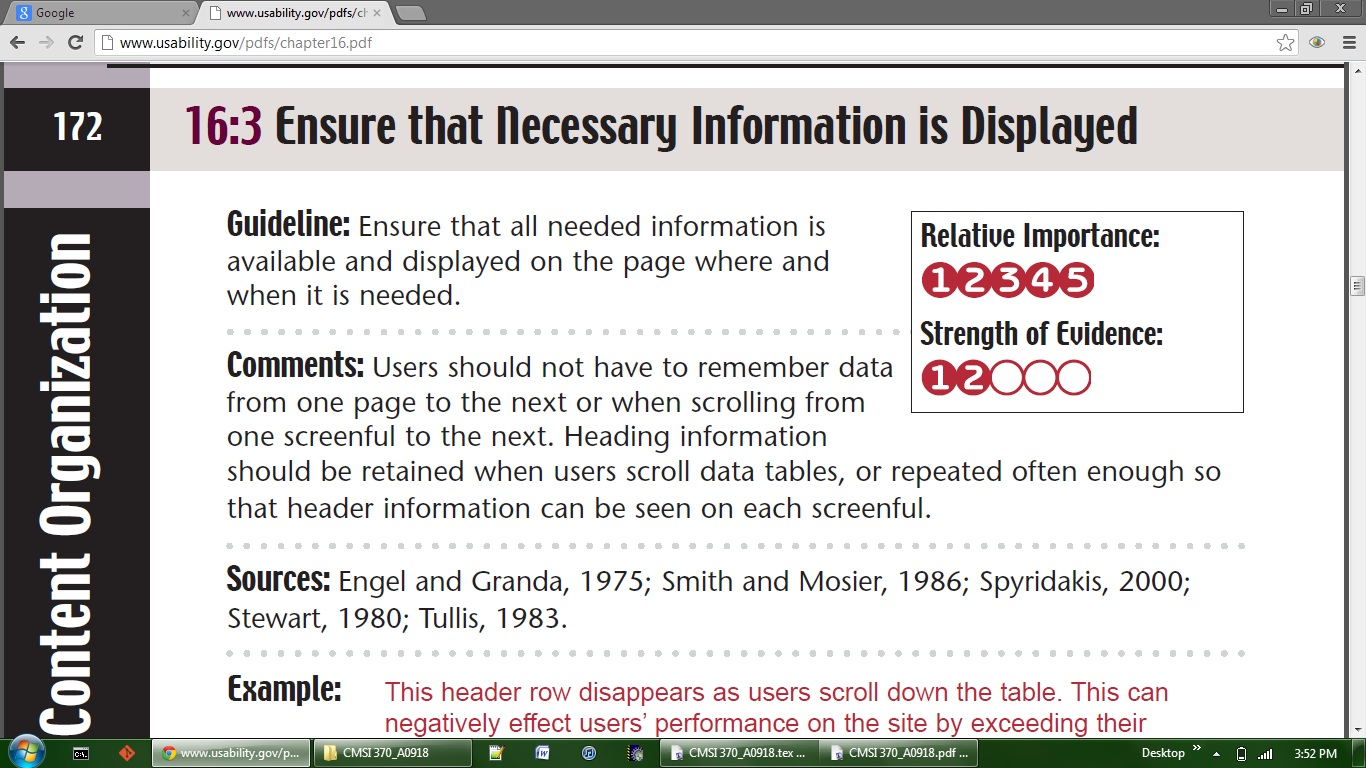
\includegraphics[width=3in]{16_3_EnsureNecessaryInfo.jpg}
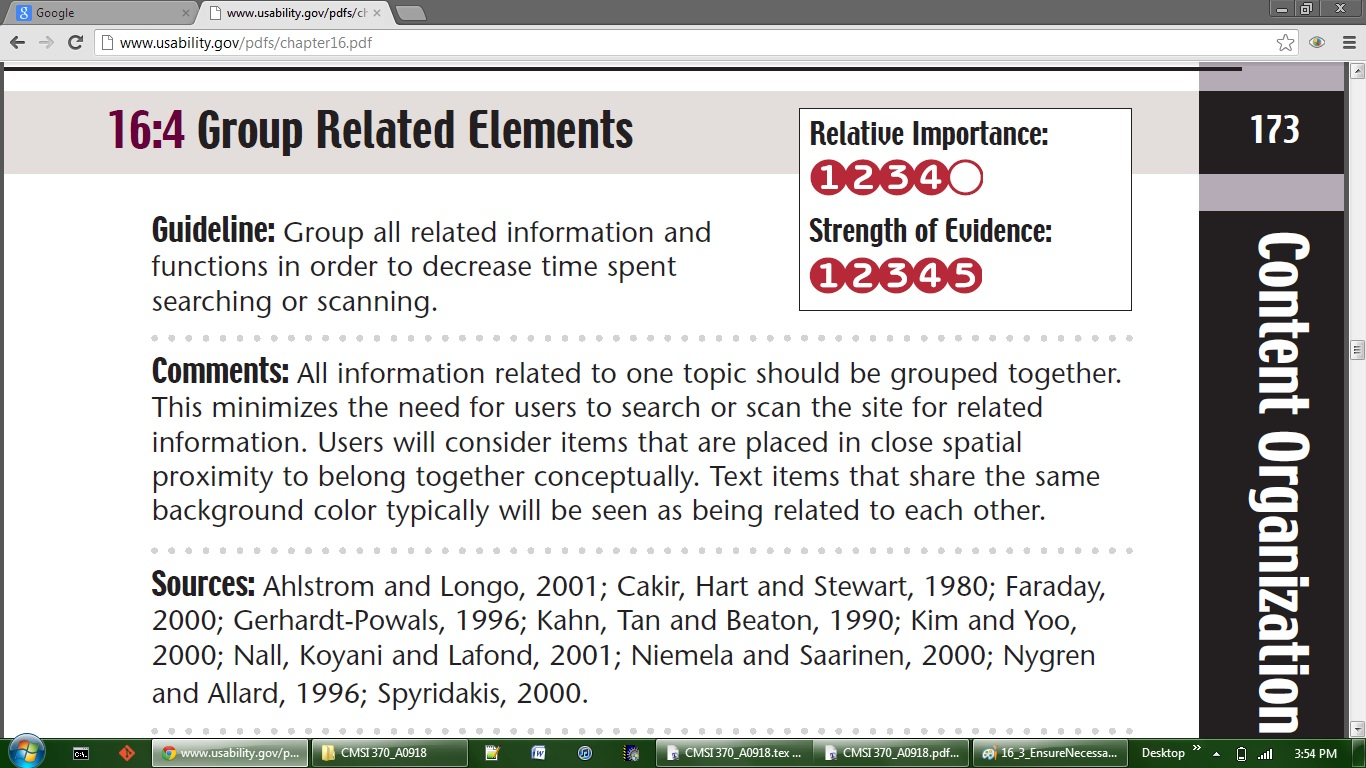
\includegraphics[width=3in]{16_4_GroupRelatedElements.jpg}


\underline{HBOGO:}
 The first guideline tries to ensure that the website displays the necessary information for the user. HBO GO seems to accomplish this task very well. The simplistic design to the homepage and the homepage displays all of the required categories a user would think of when going to the site. (i.e. movies, series, search bar, etc.) The second guideline is somewhat related to the first guideline, but is more specific. It states that a website should group all related information and functions in order to decrease time spent searching or scanning. HBO GO's homepage groups all the movies in the movies section, TV shows in the series section, etc. The website complies with this guideline very well.

\underline{Netflix:}
For the first guideline, Netflix complies with it reasonable well, however, the homepage required many clicks to get to the necessary information or displays the required information in weird ways. It tries to speed up selecting a movie by putting related movies to the ones just watched on the homepage, but this just adds more clutter. This website seems to focus more on the medium the movie is watched (i.e. dvd, online, a video queue, etc.) while most people go to Netflix to watch a movie not make these types of choices.
The elements on Netflix's homepage show ways of navigating to what the user wants, however, the website shows related movies and tv shows to the ones the user recently watched, which may or may not be what the user intended to watch. Because of this, Netflix complies with the second guideline reasonably, but not the best.

\underline{Metrics Vs. Guidelines:}
Learnability is the time it takes a user to learn a system and for this project, the time it took a new user to complete a task. Both of the guidelines I am analyzing contribute to this time. Efficiency and Satisfaction are also effected by the guidelines above, because how fast a familiar user completes the same task and the overall user satisfaction with the design of the site are based upon if HBO GO and Netflix were successful in keeping to the guidelines, two of which are stated above.






\end{document}

